\documentclass{article}

\usepackage{graphicx}
\usepackage[T1]{fontenc}


\title{Lab 6}
\author{Filip Jędrzejewski}

\begin{document}
	\maketitle
	
	\section*{Zadanie 1}
	
	\subsection*{Opis problemu}
	
	Celem zadania było wyznaczanie wartości $\pi$ wykorzystując następujący wzór:

	\begin{equation}
		\int_{0}^{1} \frac{4}{1 + x^2} \,dx = \pi
	\end{equation}

	Całkę po lewej stronie równosci wyznaczano numerycznie otrzymując przybliżone wartości $\pi$, na podstawie których badano różne metody całkowania numerycznego.	
	

	\subsection*{Całkowanie numeryczne}

	Całkę z równania (1) wyznaczano korzystając ze złożonych kwadratur prostokątów, trapezów i Simpsona. Na przedziale całkowania rozmieszczono $n = 2^m+1$ równoodległych węzłów.
	Na każdym przedziale pomiędzy dwoma sąsiednimi węzłami wyznaczno wartość całki, w zależności od metody, korzystając ze wzorów:

	\begin{equation}
		M(f) = (b-a) \cdot f \left(\frac{a+b}{2}\right)
	\end{equation}

	\begin{equation}
		T(f) = \frac{b-a}{2} \cdot (f(a) + f(b))
	\end{equation}

	\begin{equation}
		S(f) = \frac{b-a}{6} \cdot \left[ f(a) + 4 \cdot f \left(\frac{a+b}{2}\right) + f(b)\right]
	\end{equation}

	przy czym: $M(f)$ - metoda średnich prostokątów, $T(f)$ - metoda trapezów, $S(f)$ - metoda Simpsona, $a$ - początek pojedynczego przedziału, $b$ - koniec pojedynczego przedziału. 
	
	W kolejnych próbach $m$ zwiększano o $1$ (między każde dwa sąsiednie węzły dodawany był nowy węzeł). Przyjęto zakres wartości $m$ od $1$ do $25$.

	\subsection*{Wykresy}

	Dla każdej metody stworzono wykres wartości bezwzględnej błędu względnego w zależności od $m$. Wyniki przedstawiono na wspólnym wykresie, użwając skali logarytmicznej na osi $y$. 

	\begin{figure}[h]
		\centering
		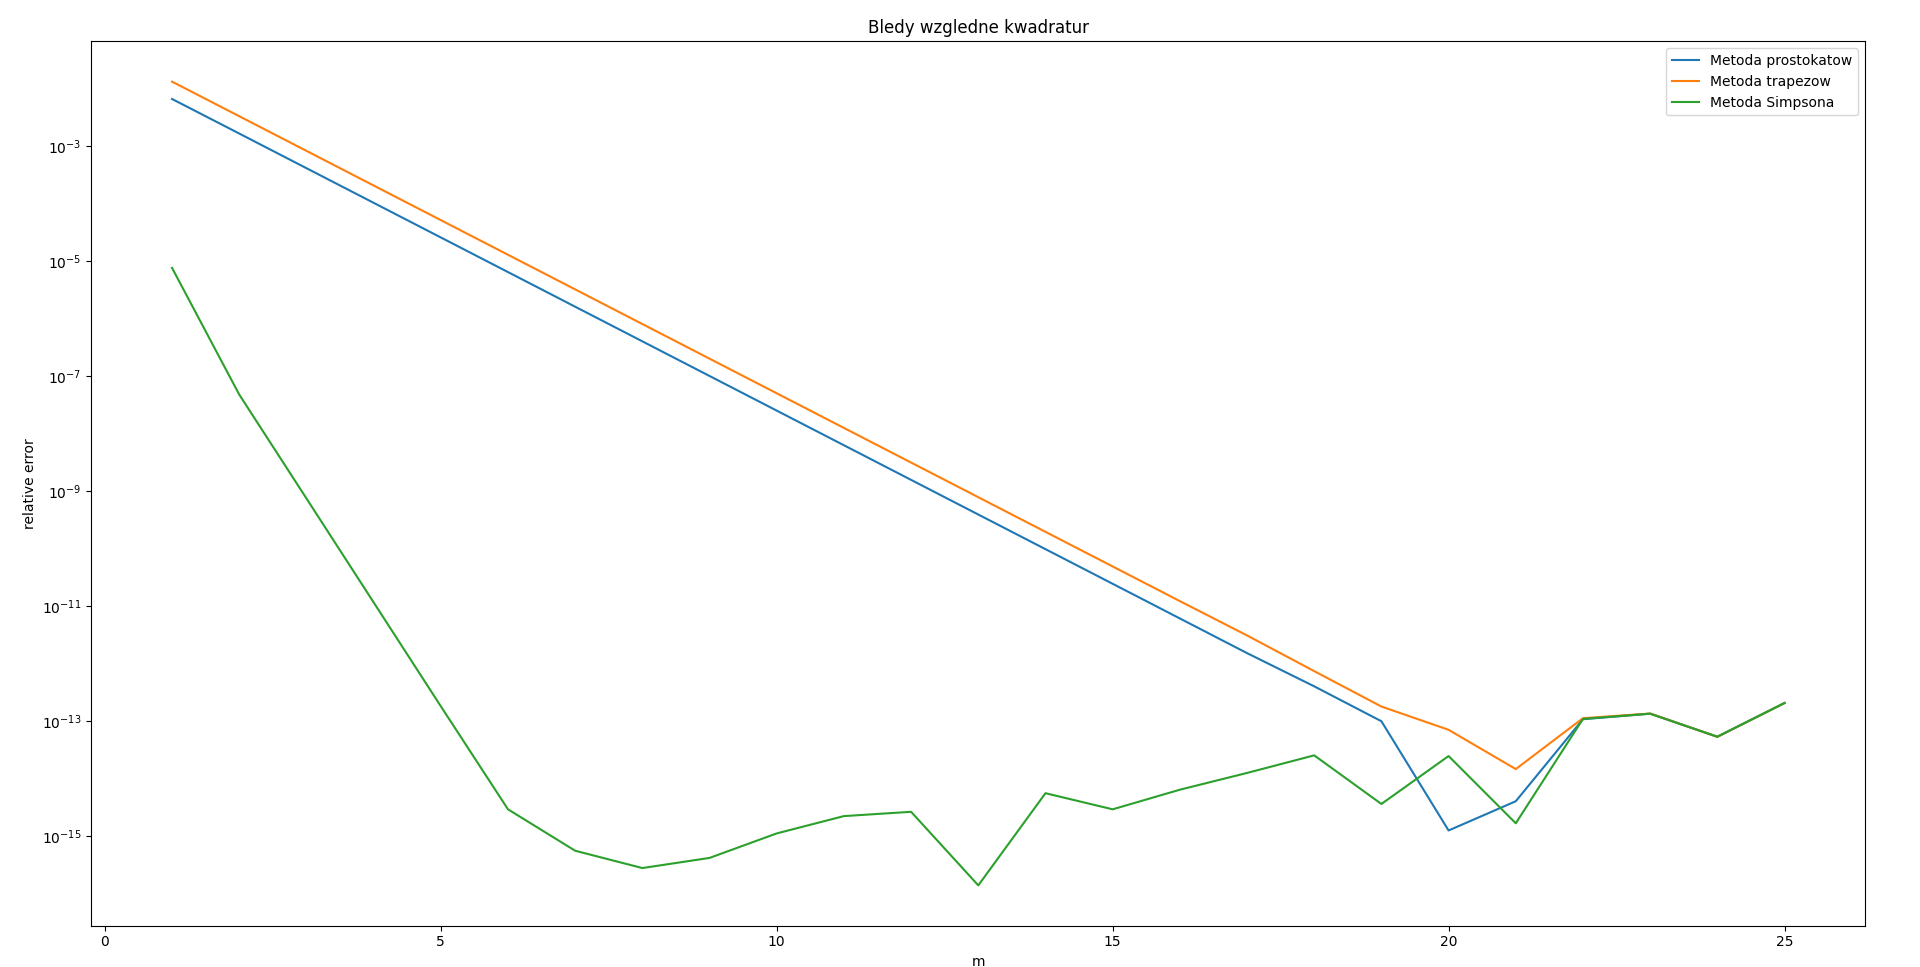
\includegraphics[scale = 0.3]{wykres1.png}
	\end{figure}


	\subsection*{Analiza wyników}

	Zauważono, że dla każdej zastosowanej metody całkowania numerycznego, istnieje pewna wartość $m_{min}$, dla której kwadratura ma najmniejszy błąd względny. Dla $m > m_{min}$ błąd kwadratury znów zaczyna rosnąć. Wartości $m_{min}$ odpowiada pewna długość kroku $h_{min}$ wyznaczona z zależności:

	\begin{equation}
		h = \frac{1}{2^m} = 2^{-m}
	\end{equation}

	Wartości $m_{min}$ oraz $h_{min}$ dla każdej z kwadratur przedstawiono w tabeli:

	\begin{center}
		\begin{tabular}{c|c|c}
  			\hline 
  			Kwadratura & $m_{min}$ & $h_{min}$ \\
			\hline
			Prostokątów & $20$ & $9,54 \cdot 10 ^ {-7}$ \\
			Trapezów & $21$ & $4,77 \cdot 10 ^ {-7}$ \\
			Simpsona & $13$ & $1,22 \cdot 10 ^ {-4}$ \\
			
		\end{tabular} 
		
	\end{center}	

	Podczas laboratorium 1 otrzymano następującą teoretyczną wartość $h_{min}$ :

	\begin{equation}
		h_{min - teoretyczne} = 1,48 \cdot 10 ^{-8}
	\end{equation}

	Wartości $h_{min}$ dla kwadratur prostokątów i trapezów większe od wartości $h_{min-teoretyczne}$ około 50 - 100 razy większe. Natomiast $h_{min-Simpsona}$ jest około 10000 razy większe od $h_{min-teoretyczne}$.


	\subsection*{Rzędy zbieżności}

	Dla każdej metody wyznaczono empiryczny rząd zbieżności dla każdej pary $h_1$, $h_2$ następujących po sobie długości kroków. W tym celu korzystano ze wzoru:

	\begin{equation}
		p \approx \frac{\log \left(\frac{E(h_2)}{E(h_1)}\right)}{\log \left(\frac{h_2}{h_1}\right)}
	\end{equation}

	przy czym: $p$ - empiryczny rząd zbieżności, $E(h)$ - błąd względny kwadratury dla danej długości kroku, $h_1$, $h_2$ - długości kroków ($h_1 > h_2$). Aby obliczenia miały sens, wartości $h_1$ i $h_2$ wybierano z przedziału, gdzie błąd metody przeważał nad błędem numerycznym. Wartości rzędów zbieżności przedstawiono na wspólnym wykresie:

	\begin{figure}[h]
		\centering
		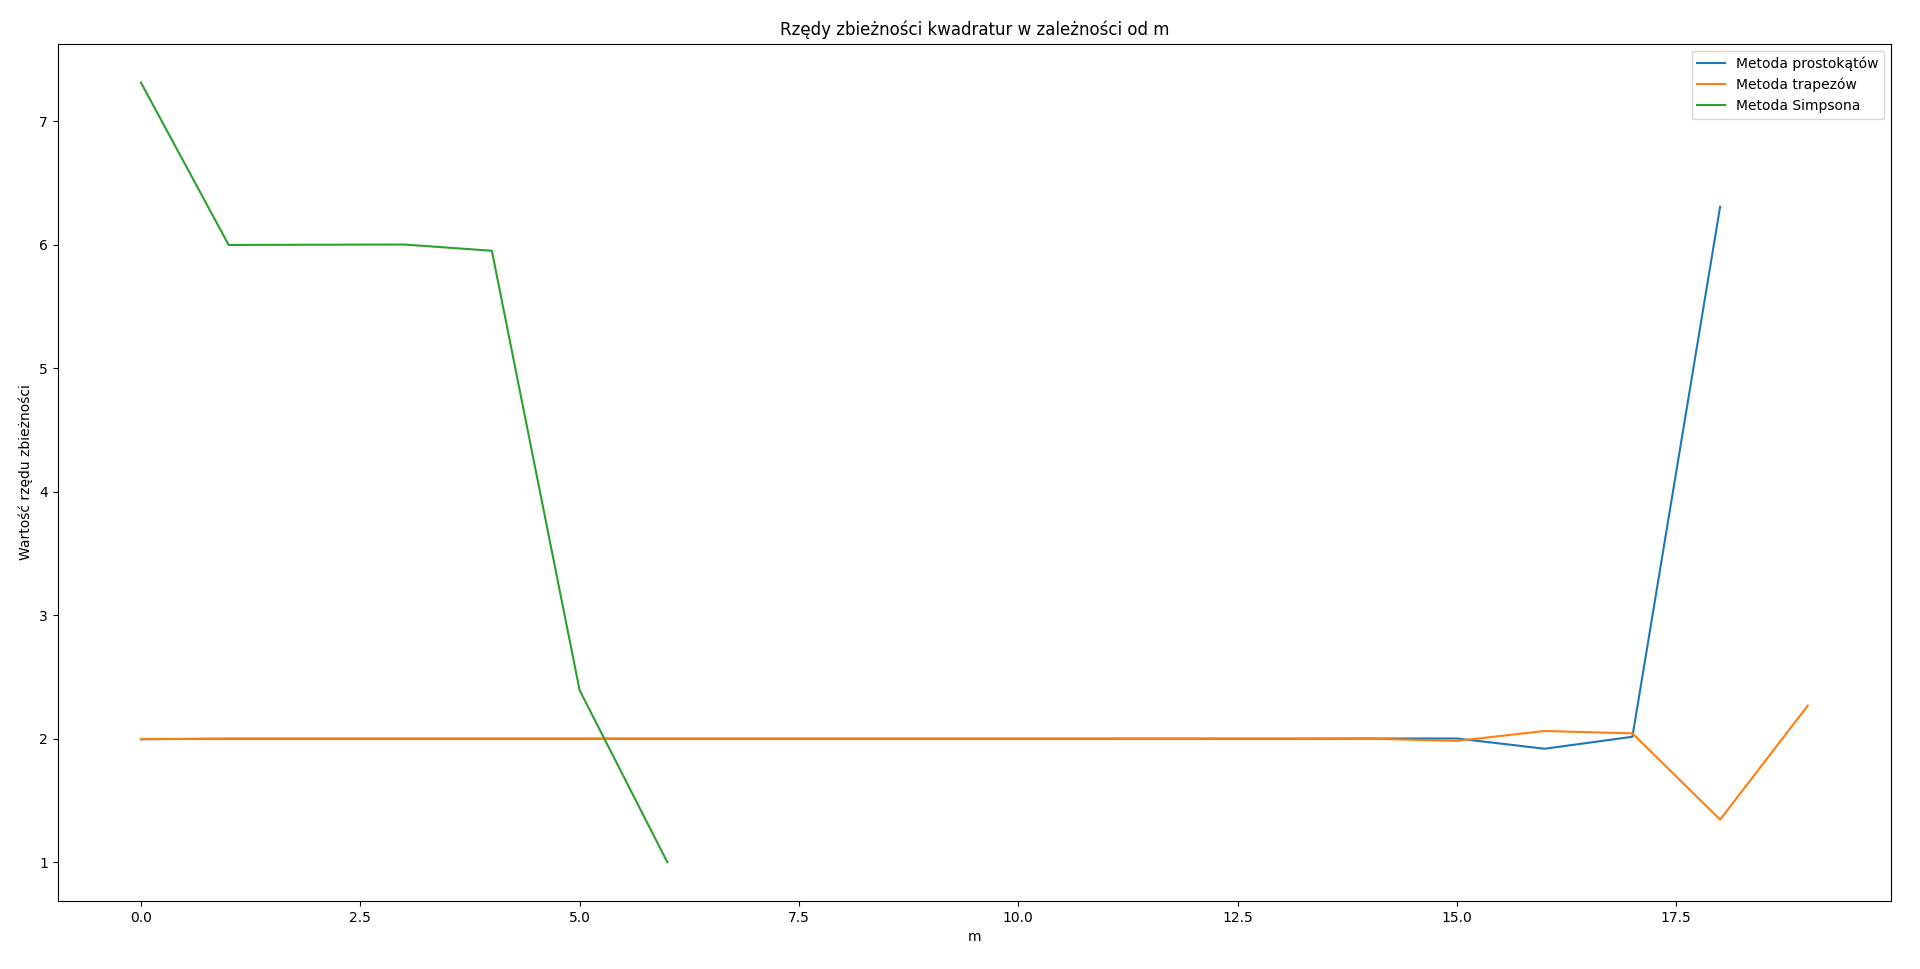
\includegraphics[scale = 0.3]{wykres2.png}
	\end{figure}
	
	\newpage

	\section*{Zadanie 2}

	\subsection*{Opis problemu}

	Celem zadania było obliczenie wartości całki:

	\begin{equation}
		\int_{0}^{1} \frac{4}{1 + x^2} \,dx 
	\end{equation}

	metodą Gaussa-Legendre'a.
	
	
	\subsection*{Całkowanie numeryczne}

	Domyślnie kwadratura Gaussa-Legendre'a działa na przedziale $[-1, 1]$, zatem na początku należało ją przeskalować na przedział $[0,1]$. 

	Na potrzeby skalowania wag użyto wzoru:

	\begin{equation}
		w_{new} = \frac{b - a}{2} \cdot w_{old}
	\end{equation}

	Natomiat na potrzeby skalowania węzłów użyto zależności:

	\begin{equation}
		x_{new} = \frac{(b - a) \cdot x_{old} + a + b}{2}
	\end{equation}

	Wzór kwadratury Gaussa-Legendre'a:

	\begin{equation}
		\int_{a}^{b} f(x) \,dx \approx \sum_{i=1}^{n} w_i f(x_i)
	\end{equation}

	W celu obliczenia całki (8) połączono wzory (9), (10) i (11) w pojedynczą funkcję:
	

	\begin{verbatim}
		import scipy.special as scis
		def gaussLegendreQuadrature(f, a, b, n):
    roots, weights = scis.roots_legendre(n)

    #obliczanie wartosci calki
    result = 0
    for i in range(len(roots)):
        x = ((b-a) * roots[i] + a + b) / 2
        w = (b-a) * weights[i] / 2
        result += w * f(x)
    
    #return wyniku
    return result
	\end{verbatim}

	\subsection*{Wykresy}

	Na podstawie funkcji z poprzedniej sekcji wyznaczano wartości całki (8) dla $n$ z zakresu od $1$ do $499$. Za pomocą tych wartości i znanego oczekiwanego wyniku ($\pi$), obliczano wartość bezwzględną błędu względnego dla każdego $n$. Na podstawie tych danych stworzono wykres:

	\begin{figure}[h]
		\centering
		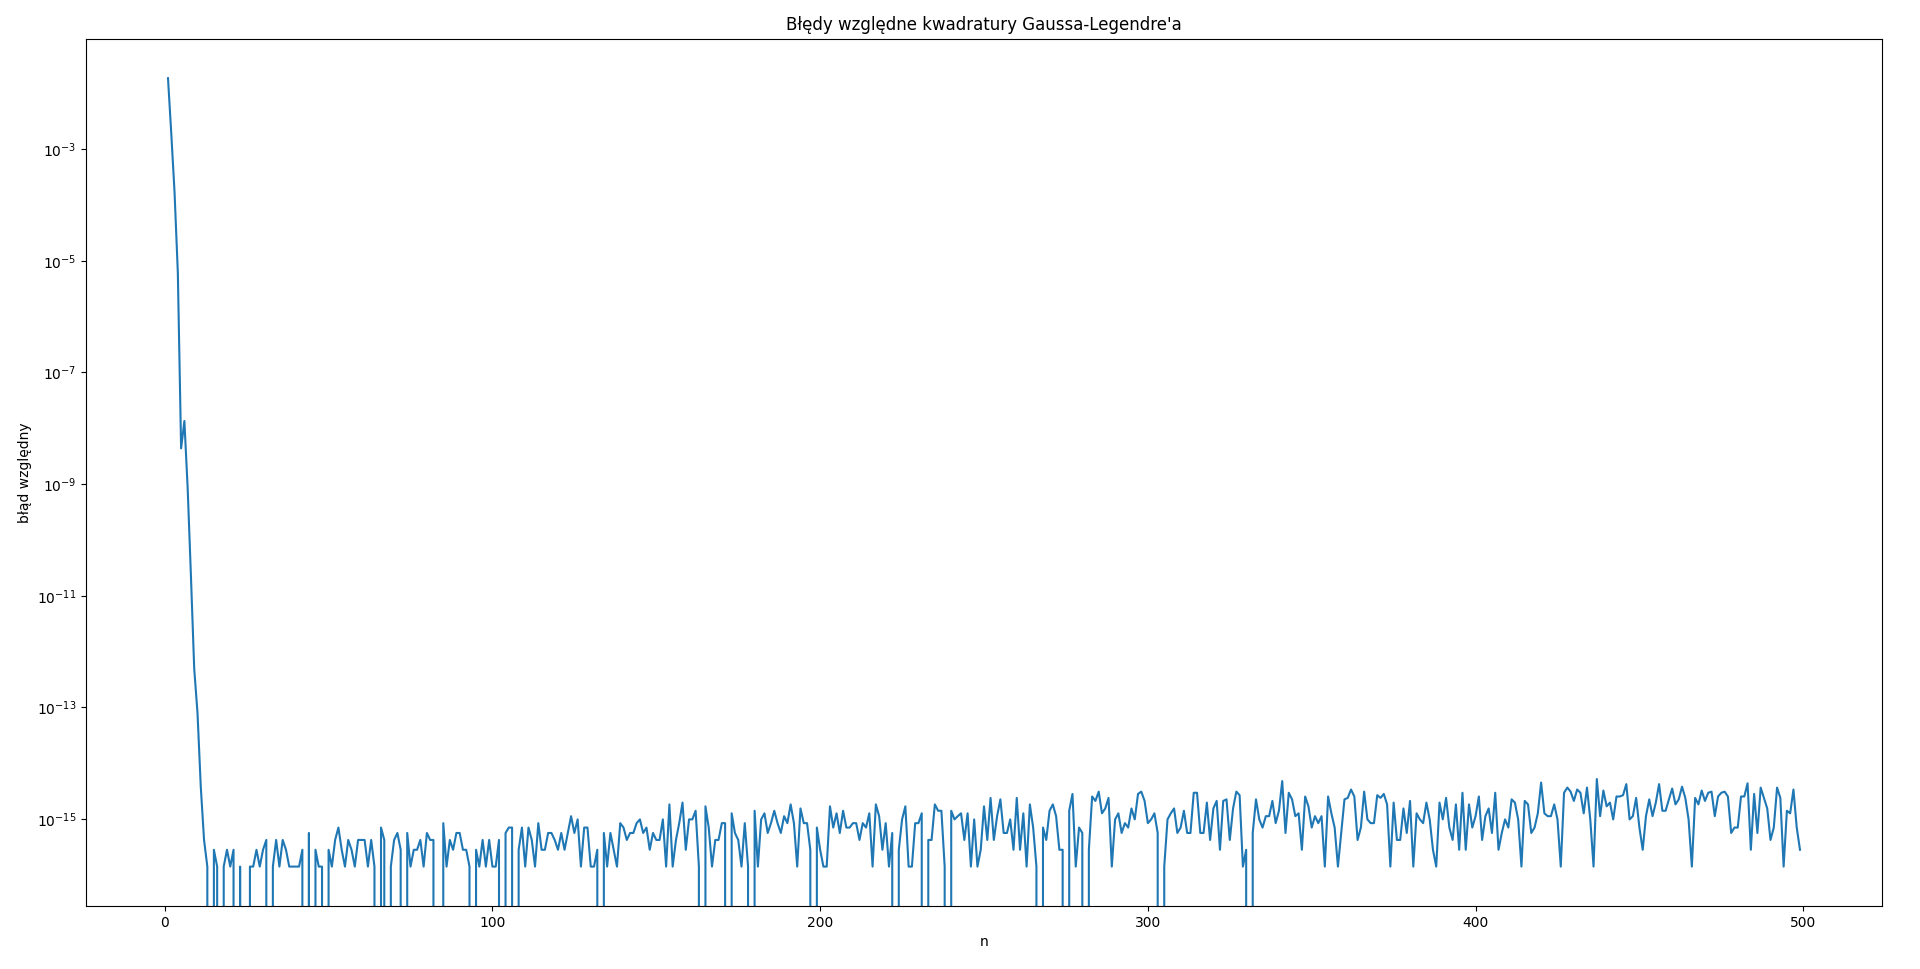
\includegraphics[scale = 0.2]{wykres3.png}
	\end{figure}


	W celu dołączenia danych z tego zadania do wykresu z zadania 1, należało przeliczyć liczbę ewaluacji $n$ na $m$ za pomocą wzoru:

	\begin{equation}
		m = \log_2 (n - 1)
	\end{equation}


	W tej formie dodano wyniki z tego zadania do wykresu z zadania 1:

	\begin{figure}[h]
		\centering
		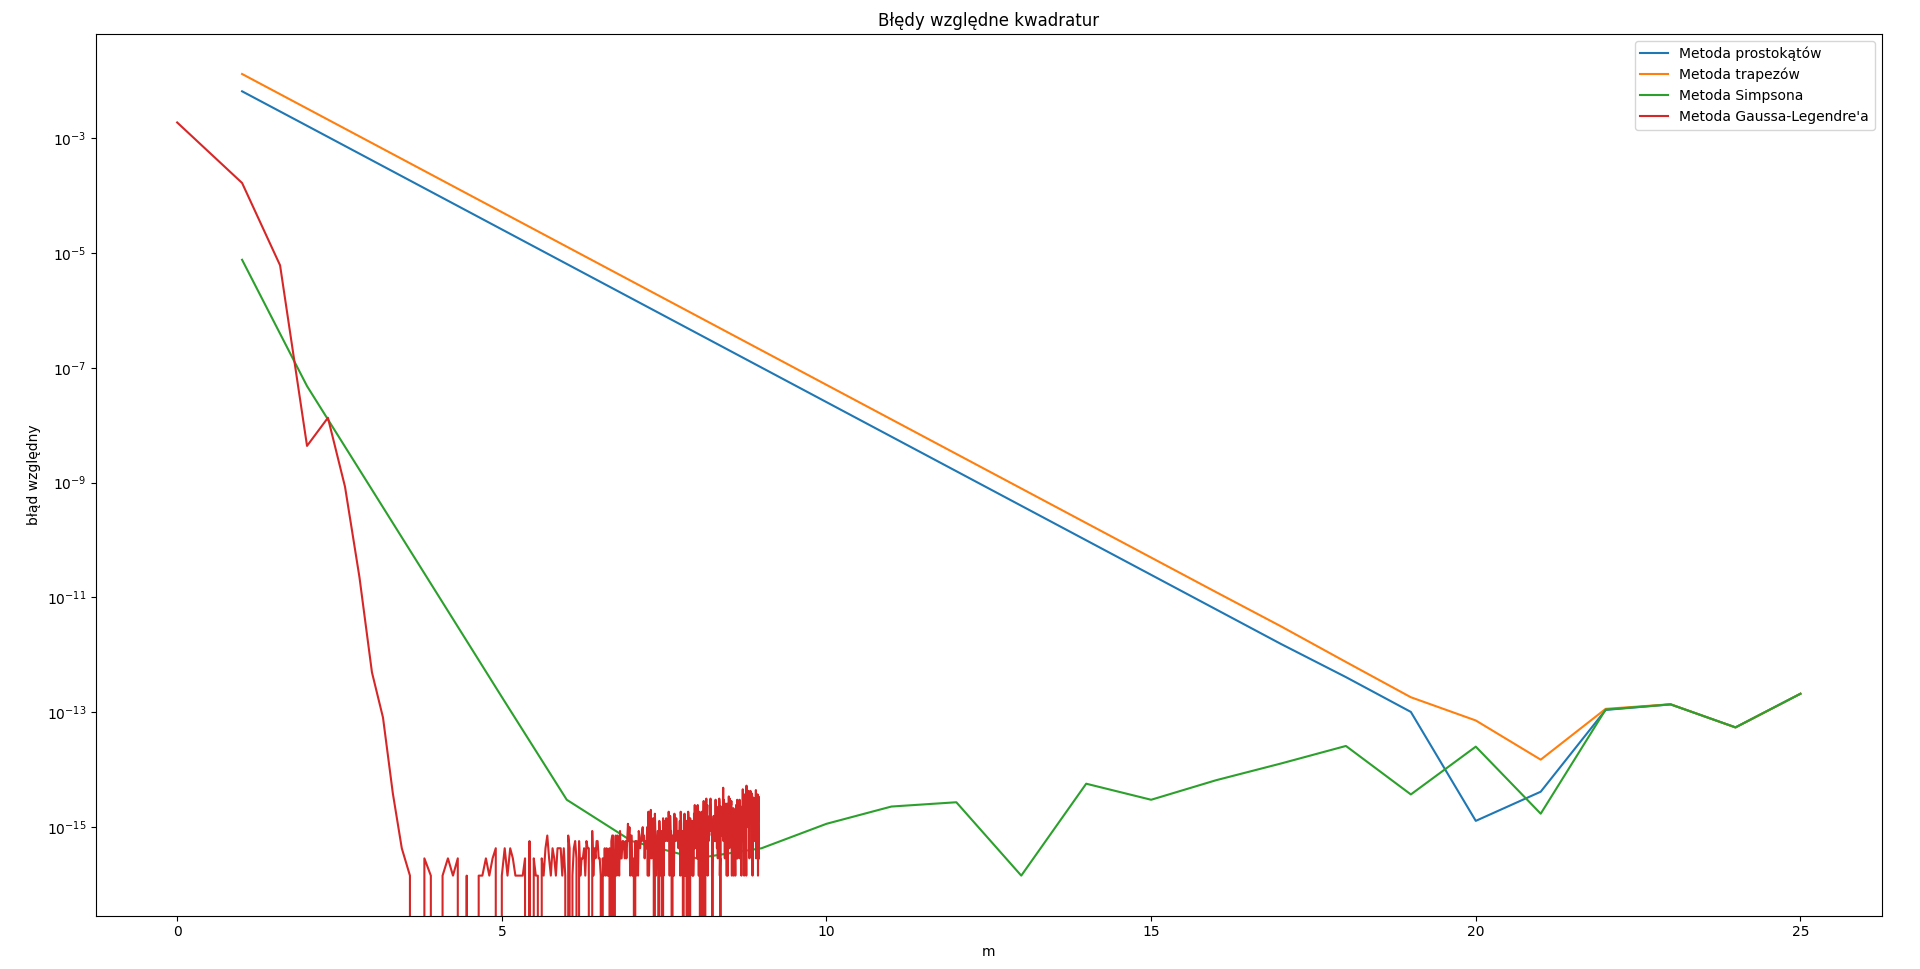
\includegraphics[scale = 0.3]{wykres4.png}
	\end{figure}


	Na wykresie dobrze widać, jak błąd numeryczny zaczyna przeważać nad błędem metody Gaussa-Legendre'a.
	
	
	
	
	
	
	
	
	
	
	
	
	
	
	
	
	
	
	
\end{document}